\setchapterstyle{lines}
\pagelayout{wide}

\chapter{Light-Cone Quantization}
\labch{appendixlc}
\section{Light-front form}
Let us begin by choosing an appropriate coordinate system, that is one which would naturally allow for both a relativistic and quantum mechanical treatment. In \cite{reldyn}, Dirac identified three possible manners of constructing such a formulation: the \textbf{\textsf{\color{ming}instant form}}, the \textbf{\textsf{\color{ming}front form}} and the \textbf{\textsf{\color{ming}point form}}. \\
The starting point for their derivation consists of the fact that a relativistic quantum system must, in an intrinsic way, possess invariance under inhomogeneous infinitesimal Lorentz transformations and also a Hamiltonian formulation. The first condition may simply be equivalently expressed as invariance under the action of the generators belonging to the Poincar\'e group, whereas the second one imposes particular transformation laws for the quantum Poisson bracket of any two dynamical variables. 

\subsubsection*{The instant form}
Given the Minkowski space-time equipped with a metric
\begin{align*}
g_{\mu\nu}=g^{\mu\nu}=
\left( \begin{array}{cccc}
1 & 0  & 0  & 0\\
0 & -1 & 0  & 0\\
0 & 0  & -1 & 0\\
0 & 0  & 0  & -1\end{array} \right),
\end{align*}
the instant form is simply characterized by the usual covariant coordinates
\begin{align*}
x^\mu=(x^0,\underbrace{x^1,x^2}_{\overset{\Delta}{=} \vec{x}_\perp},x^3)=(x^0,\vec{x}_\perp,x^3).
\end{align*}
Using a similar notation, the contravariant $x_\mu=(x_0,\vec{x}_\perp,x_3)$ may be expressed as $x_\mu=g_{\mu\nu}x^\nu=(x^0,-\vec{x}_\perp,-x^3)$. The scalar product is simply given by
\begin{align*}
x\cdot y=x_\mu y^\mu=g_{\mu\nu}x^\mu y^\mu=x^0y^0-\underbrace{(x^1y^1+x^2y^2)}_{\vec{x}_\perp\cdot \vec{y}_\perp}-x^3y^3.
\end{align*}

\begin{figure*}[!h]
\captionsetup[subfigure]{justification=centering}
\begin{subfigure}{.49\textwidth}
  \centering
  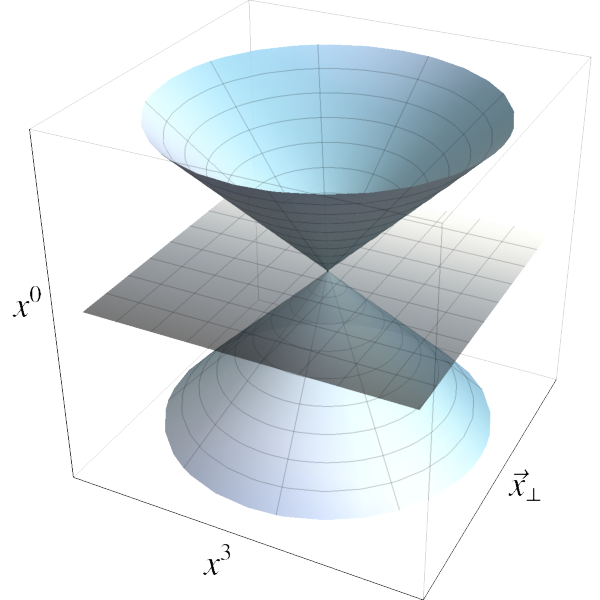
\includegraphics[width=.9\linewidth]{lc_1.pdf}  
  \caption*{\normalsize The instant form initialized at $x^0=0$.}   
\end{subfigure}
\begin{subfigure}{.49\textwidth}
  \centering
  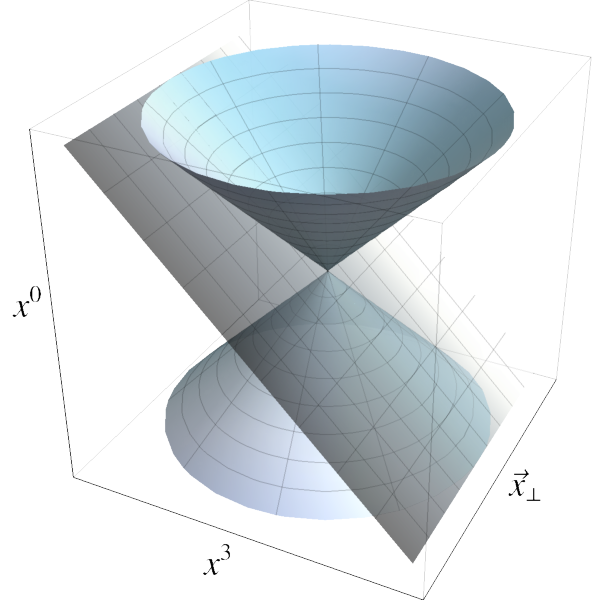
\includegraphics[width=.9\linewidth]{lc_2.pdf}  
  \caption*{\normalsize The front form initialized at $x^+=0$.}
\end{subfigure}
% \caption{Put your caption here}
\end{figure*}

\subsubsection*{\sffamily Transition to other forms}
Let us enforce a clear separation between the time and spatial coordinates by introducing the notation
\begin{align*}
x^\mu=(x^0=t,\underbrace{x^1,x^2,x^3}_{\overset{\Delta}{=}\mathbf{x}})=(t,\mathbf{x}).
\end{align*}
The evolution of a system characterized by a wavefunction $\Psi(t,\mathbf{x})$ is given by the Schr\"{o}dinger equation
\begin{align*}
H_0\Psi(t,\mathbf{x})=i\frac{\partial}{\partial t}\Psi(t,\mathbf{x}),
\end{align*}
where the free Hamiltonian $H_0$ represents the generator of spatial translations along $\mathbf{x}$ in the time $t$. The solution for the above equation is obtained after imposing initial conditions $\Psi(t_0,\mathbf{x}_0)$ on a space-like hypersurface at $t=0$.\\
One may adopt a more general approach and use generic coordinates $\widetilde{x}^\mu=(\widetilde{x}^0,\widetilde{\mathbf{x}})$. A similar evolution equation for the state $\Psi(\widetilde{x}^0,\widetilde{\mathbf{x}})$ may also be written as
\begin{align*}
\widetilde{H}_0\Psi(\widetilde{x}^0,\widetilde{\mathbf{x}})=i\frac{\partial}{\partial \widetilde{x}^0}\Psi(\widetilde{x}^0,\widetilde{\mathbf{x}}),
\end{align*}
with the initial conditions $\Psi(\widetilde{x}^0,\widetilde{\mathbf{x}})$ expressed on a null-time hypersurface $\widetilde{x}^0=0$. \\
Each specific choice of coordinates provides a certain equation for the null-time hypersurface, which then describes a certain form of relativistic quantum mechanics. These choices of coordinates must be independent of each other, in the sense that one may not obtain a parametrization from another via a Lorentz transformation \cite{mantovani}. \\ 
Besides the three forms of relativistic dynamics identified by Dirac, there are another two, chosen such that they satisfy the requirements: there exist a subgroup from the Poincar\'e generators which leave the hypersurface invariant; they act in such a way that any points from the hypersurface may be connected via a transformation from the group of these generators \cite{heinzl}. In the following, we shall focus on the light-front form. 

\subsubsection*{\sffamily The front form}
Let us perform a change of variables $(x^0,\vec{x}_\perp,x^3)\mapsto (x^+\vec{x}_\perp,x^-)$ and introduce the light-cone coordinates
\begin{align*}
x^\pm\overset{\Delta}{=}\frac{1}{\sqrt{2}}\left(x^0\pm x^3\right),
\end{align*}
A simple manipulation lead to an expression for the scalar product
\begin{align*}
x\cdot y &= x^0y^0-x^3y^3-\vec{x}_\perp\cdot\vec{y}_\perp\\
&=\frac{1}{2}\left[(x^0+x^3)(y^0-y^3)+(x^0-x^3)(y^0+y^3)\right]-\vec{x}_\perp\cdot\vec{y}_\perp\\
&=x^+y^-+x^-y^+-\vec{x}_\perp\cdot\vec{y}_\perp.
\end{align*}

We may easily conclude that the metric tensor becomes non-diagonal
\begin{align*}
\widetilde{g}_{\mu\nu}=\widetilde{g}^{\mu\nu}=
\left( \begin{array}{cccc}
0 & 0  & 0  & 1\\
0 & -1 & 0  & 0\\
0 & 0  & -1 & 0\\
1 & 0  & 0  & 0\end{array} \right).
\end{align*}
When performing integrals, the volume element only acquires a unity factor from the Jacobian associated to the change of coordinates:
\begin{align*}
\int d^4x=\int dx^+dx^-d^2\vec{x}_\perp.
\end{align*}
Even though straight-forward, let us explicitly write down how the spatial and time partial derivatives look like. For simplicity, we are going to introduce the notations
\begin{equation*}
\begin{aligned}
\partial_\alpha\overset{\Delta}{=}\frac{\partial}{\partial x^\alpha}, &&
\partial^\alpha\overset{\Delta}{=}\frac{\partial}{\partial x_\alpha},
\end{aligned}
\end{equation*}
where the index $\alpha=\big\{+,-,\perp\big\}$. Hence, we have
\begin{align*}
\partial_+&=\widetilde{g}^{+-}\partial^-=\partial^-,\\
\partial_-&=\widetilde{g}^{-+}\partial^+=\partial^+,\\
\partial_i&=\widetilde{g}^{ij}\partial^j=-\partial^i, \text{ where }i,j=1,2.
\end{align*}

\begin{equation*}
\def\arraystretch{1.3}
\begin{array}{@{}lll@{}}
\toprule
 \multicolumn{3}{c@{}}{\text{Kinematic comparison between the instant and light-front forms}} \\
\cmidrule{1-3}
 \text{time coordinate} & x^0 & x^+\\
 \text{spatial coordinates} & (\vec{x}_\perp,x^3) & (\vec{x}_\perp,x^-)\\
 \text{metric tensor} & \begin{aligned}[t]g^{00}&=1,\\
 g^{11}&=g^{22}=g^{33}=-1 \end{aligned}& \begin{aligned}[t]&\widetilde{g}^{+-}=\widetilde{g}^{-+}=1,\\&\widetilde{g}^{11}=\widetilde{g}^{22}=-1\end{aligned}\\
 \text{scalar product} & x^0y^0-x^3y^3-\vec{x}_\perp\cdot\vec{y}_\perp& x^+y^-+x^-y^+-\vec{x}_\perp\cdot\vec{y}_\perp\\
 \text{time derivative} & \partial_0=\partial^0 & \partial_+=\partial^-\\
  \text{spatial derivatives} & \partial_i=-\partial^i, \text{ }i=1,2,3 & \partial_-=\partial^+,\partial_i=-\partial^i, \text{ }i=1,2\\
\bottomrule
\end{array}
\end{equation*}

\section{Poincar\'e on the light-cone}
Any form of relativistic quantum mechanics is constructed using the Poincar\'e group $\mathbb{R}\times \mathcal{SO}(1,3)$. The associated Lie algebra is given by the commutation relations
\begin{equation}
\label{lc1}
\begin{aligned}
&[P^\nu,P^\mu]=0,\\
&[M^{\nu\mu},P^\rho]=i(g^{\nu\rho}P^\mu-g^{\nu\rho}P^\mu),\\
&[M^{\nu\mu},M^{\rho\sigma}]=i(g^{\nu\sigma}M^{\mu\rho}-g^{\nu\rho}M^{\mu\sigma}+g^{\mu\rho}M^{\nu\sigma}-g^{\mu\sigma}M^{\nu\rho}),
%\coloredlabel
\end{aligned}
\end{equation}
where $P^\nu$ are spatial translations and $M^{\nu\mu}$ Lorentz transformations. If we introduce
\begin{align*}
J^i\overset{\Delta}{=}\epsilon^{ijk}M^{jk}, && K^i\overset{\Delta}{=}M^{0i},
\end{align*}
the expressions written in Equation~(\cref{lc1}) become
\begin{equation*}
\begin{aligned}
&[J^i,P^j]=i\epsilon^{ijk}P^k, && [J^i,J^j]=i\epsilon^{ijk}J^k,\\ 
&[J^i,P^0]=0, && [J^i,K^j]=i\epsilon^{ijk}K^k, \\ 
&[K^i,P^j]=-i\delta^{ij}P^0, && [K^i,K^j]=-i\epsilon^{ijk}J^k, \\ 
&[K^i,P^0]=-iP^i,
\end{aligned}
\end{equation*}
from which we may infer that $J^i$ generate rotations, whereas $K^i$ is a boost operator. \\
In light-cone coordinates, the generators of the Poincar\'e algebra are \cite{qedimf}
\begin{equation}
\label{lc2}
\begin{aligned}[t]
\widetilde{P}^\mu=(P^+,P^1,P^2,P^-),
%\coloredlabel
\end{aligned}
\qquad
\begin{aligned}[t]
\widetilde{M}^{\nu\mu}=\left( \begin{array}{cccc}
0 & -S^1  & -S^2  & K^3\\
 S^1 &    0 &  J^3 & B^1\\
 S^2 & -J^3 &    0 & B^2\\
-K^3 & -B^1 & -B^2 &   0\end{array} \right),
\end{aligned}
\end{equation}
where we introduced the notations
\begin{equation}
\label{lc3}
\begin{aligned}
&  P^+\overset{\Delta}{=}\frac{P^0+P^3}{\sqrt{2}},
&& B^1\overset{\Delta}{=}\frac{K^1+J^2}{\sqrt{2}},
&& S^1\overset{\Delta}{=}\frac{K^1-J^2}{\sqrt{2}}\\
&  P^-\overset{\Delta}{=}\frac{P^0-P^3}{\sqrt{2}},
&& B^2\overset{\Delta}{=}\frac{K^2-J^1}{\sqrt{2}},
&& S^2\overset{\Delta}{=}\frac{K^2+J^1}{\sqrt{2}}.
%\coloredlabel
\end{aligned}
\end{equation}

\begin{note}
\noindent
In order to deduce how the Poincar\'e generators transform under the change of coordinates $x^\alpha=(x^0,x^1,x^2,x^3)\mapsto  \widetilde{x}^\mu=(x^+,x^1,x^2,x^-)$, we first compute the matrix associated to the transformation $\widetilde{x}^\mu=C_\alpha^\mu x^\alpha$ as
\begin{align*}
C_\alpha^\mu=\frac{1}{\sqrt{2}}\left( \begin{array}{cccc}
1 & 0 & 0 & 1\\
0 & \sqrt{2} & 0 & 0\\
0 & 0 & \sqrt{2} & 0\\
1 & 0 & 0 & -1\end{array} \right).
\end{align*}
Hence, the four momentum, which is a four-vector, transforms as
\begin{align*}
\widetilde{P}^\mu&=C_\alpha^\mu P^\alpha=\left( \begin{array}{cccc}
\frac{1}{\sqrt{2}} & 0 & 0 & \frac{1}{\sqrt{2}}\\
0 & 1 & 0 & 0\\
0 & 0 & 0 & 1\\
\frac{1}{\sqrt{2}} & 0 & 0 & -\frac{1}{\sqrt{2}}\end{array} \right)(P^0,P^1,P^2,P^3)=\left(\frac{P^0+P^3}{\sqrt{2}},P^1,P^2,\frac{P^0-P^3}{\sqrt{2}}\right)
\end{align*}
Similarly, a four-tensor of second rank will transform according to
\begin{align*}
\widetilde{M}^{\mu\nu}&=C_\alpha^\mu M^{\alpha\beta}\left(C_\beta^\nu\right)^T\\
&=\left( \begin{array}{cccc}
\frac{1}{\sqrt{2}} & 0 & 0 & \frac{1}{\sqrt{2}}\\
0 & 1 & 0 & 0\\
0 & 0 & 0 & 1\\
\frac{1}{\sqrt{2}} & 0 & 0 & -\frac{1}{\sqrt{2}}\end{array} \right)
\left( \begin{array}{cccc}
0 & -K^1 & -K^2 & -K^3\\
K^1 & 0 & J^3 & -J^2\\
K^2 & -J^3 & 0 & J^1\\
K^3 & J^2 & -J^1 & 0\end{array} \right)
\left( \begin{array}{cccc}
\frac{1}{\sqrt{2}} & 0 & 0 & \frac{1}{\sqrt{2}}\\
0 & 1 & 0 & 0\\
0 & 0 & 0 & 1\\
\frac{1}{\sqrt{2}} & 0 & 0 & -\frac{1}{\sqrt{2}}\end{array} \right)\\
&=\left( \begin{array}{cccc}
0 & -\frac{K^1-J^2}{\sqrt{2}} & -\frac{K^2+J^1}{\sqrt{2}} & K^3\\
\frac{K^1-J^2}{\sqrt{2}} & 0 & J^3 & \frac{K^1+J^2}{\sqrt{2}}\\
\frac{K^2+J^1}{\sqrt{2}} & -J^3 & 0 & \frac{K^2-J^1}{\sqrt{2}}\\
-K^3 & -\frac{K^1+J^2}{\sqrt{2}} & -\frac{K^2-J^1}{\sqrt{2}} & 0\end{array} \right).
\end{align*}
All the above results, after making use of the notations from Equation~(\cref{lc3}), lead exactly to the expected results given in Equation~(\cref{lc2}).
\end{note}

Hence, the generators of the Poincar\'e group in the light-front framework may schematically be written as
\begin{equation}\label{lc36}
\begin{aligned}
\left\lbrace \widetilde{P}^\mu\overset{\Delta}{=}(P^+,\vec{P}_\perp,P^-),\vec{B}_\perp\overset{\Delta}{=}(B^1,B^2),\vec{S}_\perp\overset{\Delta}{=}(S^1,S^2),J^3, K^3\right\rbrace
\end{aligned}
\end{equation}

\subsubsection*{\sffamily Two-dimensional Galilean sub-group structure}
One important feature of the light-front parametrization is that the Poincar\'e group possesses a sub-group isomorphic to the two-dimensional Galilean group. In order to explicitly see this structure, we begin by writing the commutation relations for all the light-front Poincar\'e generators
\begin{equation}
\label{lc4}
\begin{aligned}
&[P^+,P^-]=0, && [P^+,\vec{P}_\perp^i]=0,\\
&[P^+,\vec{B}_\perp^i]=0, && [P^+,J^3]=0, \\
&[P^-,\vec{P}_\perp^i]=0, && [P^-,\vec{B}_\perp^i]=i\vec{P}_\perp^i,\\
&[P^-,J^3]=0, && [\vec{P}_\perp^i,\vec{B}_\perp^j]=i\delta^{ij}P^+,\\
&[J^3,\vec{P}_\perp^i]=i\epsilon^{ij}\vec{P}_\perp^j, &&[J^3,\vec{B}_\perp^i]=i\epsilon^{ij}\vec{B}_\perp^j.
%\coloredlabel
\end{aligned}
\end{equation}

Let us now write down the defining commutators for the two-dimensional Galilei group, whose associated algebra is generated by the rotation $\mathcal{J}$, the boost along two directions $\mathcal{B}^i$, the two spatial translations $\mathcal{P}^i$, the Hamiltonian $\mathcal{H}$ and the mass $\mathcal{M}$ as
\begin{equation}
\label{lc5}
\begin{aligned}
&[\mathcal{M},\mathcal{H}]=0, && [\mathcal{M},\mathcal{P}^i]=0, \\
&[\mathcal{M},\mathcal{B}^i]=0, && [\mathcal{M},\mathcal{J}]=0, \\
&[\mathcal{H},\mathcal{P}^i]=0, && [\mathcal{H},\mathcal{B}^i]=i\mathcal{P}^i,\\
&[\mathcal{H},\mathcal{J}]=0, && [\mathcal{P}^i,\mathcal{B}^j]=i\delta^{ij}\mathcal{M},\\
&[\mathcal{J},\mathcal{P}^i]=i\epsilon^{ij}\mathcal{P}^j, &&[\mathcal{J},\mathcal{B}^i]=i\epsilon^{ij}\mathcal{B}^j.
%\coloredlabel
\end{aligned}
\end{equation}
After a direct comparison between Equations~(\cref{lc4}) and~(\cref{lc5}), one may immediately establish the correspondences: $P^+\leftrightarrow \mathcal{M}$, $P^i\leftrightarrow \mathcal{H}$, $\vec{P}_\perp^i\leftrightarrow \mathcal{P}^i$, $\vec{B}_\perp^i\leftrightarrow \mathcal{B}^i$ and $J^3\leftrightarrow \mathcal{J}$. Hence, we may conclude that indeed the Poincar\'e group consisting of $\left\lbrace \tilde{P}^\mu,\vec{B}_\perp\,\vec{S}_\perp,J^3, K^3\right\rbrace$ has a sub-group $\left\lbrace P^+,P^-,\vec{P}_\perp^i,\vec{B}_\perp^i,J^3 \right\rbrace$ who is isomorphic with the two-dimensional Galilean group. Consequently, we may assign physical interpretations of some light-cone Poincar\'e generators as
\begin{align*}
P^+&\longleftrightarrow\text{mass},\\
P^-&\longleftrightarrow\text{time translation},\\
\vec{P}_\perp^i&\longleftrightarrow\text{spatial translations},\\
\vec{B}_\perp^i&\longleftrightarrow\text{boosts},\\
J^3&\longleftrightarrow\text{rotation}.
\end{align*}

The generator $P^-$ represents the Hamiltonian of the system, and since the Hamiltonian is the generator of translations in time, we may now interpret $x^+$ as the light-cone time. \\ 
The existence of this particular isomorphism assures that the Hamiltonian expressed in these coordinates has an intrinsic non-relativistic structure \cite{susskind}. This may explicitly be seen from the dispersion relation $M^2=P_\mu P^\mu=2P^+P^--\vec{P}_\perp^2$, which then gives
\begin{align}\label{lc37}
P^-=\frac{1}{2P^+}\underbrace{\vec{P}_\perp^2+M^2}_{\overset{\Delta}{=}M^2_\perp}.
\end{align}

Let us also notice that, as a consequence of this expression, the light-cone momentum $P^+$ always has only positive values, in comparison with the momenta on the instant form which may also take negative values. This implies that the vacuum state, defined for a free theory as $a_{\vec{P}}\ket{0}=0$ in normal coordinates or $a_{P^+,\vec{P}_\perp}\ket{0}=0$ on the light-cone, becomes much simpler for an interacting theory in the light-front form. In light-cone coordinates, the vacuum may consists only excitations of the state given by $P^+=0$, whereas in general many other excited states also contribute, hence complicating its underlying structure. From this, the light-cone vacuum is said to be trivial \cite{burkardt}. This turns out to be extremely useful since one may compute, using light-cone coordinates, any interacting state by simply applying creation operators upon this trivial vacuum. 

\begin{equation*}
\def\arraystretch{1.3}
\begin{array}{@{}lll@{}}
\toprule
 \multicolumn{3}{c@{}}{\text{Comparison between generators in the instant and light-front forms}} \\
\cmidrule{1-3}
 \text{free Hamiltonian} & H=\sqrt{\vec{P}^2+M^2} & P^-=\dfrac{\vec{P}_\perp^2+M^2}{2P^+}\\
 \text{conserved quantities} & E,\vec{P} & P^-,P^+,\vec{P}_\perp\\
 \text{momenta} & P_z\in(-\infty,+\infty)& P^+\in(0,+\infty)\\
 \text{quantized Hamiltonian} & P^{0}=\sum\limits_{\vec{k}} a_{\vec{k}}^{\dagger} a_{\vec{k}} \sqrt{m^{2}+\vec{k}^{2}} & P_{+}=\sum\limits_{k_{-}, \vec{k}_{\perp}} a_{k_{-}, \vec{k}_{\perp}}^{\dagger} a_{k_{-}, \vec{k}_{\perp}} \dfrac{m^{2}+\vec{k}_{\perp}^{2}}{2 k_{-}}\\
 \text{vacuum of free theory} & a_{\vec{k}}\ket{0}=0 & a_{k_{-}, \vec{k}_{\perp}}\ket{0}=0\\
 \text{vacuum of interacting theory} & \text{many states with }\vec{P}=0 & \text{only zero-mode states }P^+=0\\
\bottomrule
\end{array}
\end{equation*}


\section{Light-cone QCD}
\subsubsection*{\sffamily Conventions}
Let us proceed by stating our conventions and notations. The gamma matrices in the usual instant form are given by
\begin{subequations}
\begin{align}
\left\lbrace\gamma^\mu,\gamma^\nu\right\rbrace&=2g^{\mu\nu}\mathds{1},\label{lc8a}%\coloredlabel
\\
{\gamma^\mu}^\dag&=\gamma^0\gamma^\mu\gamma^0 \label{lc8b}.
%\coloredlabel
\end{align}
\end{subequations}
In light-cone coordinates, they are defined as
\begin{align}
\label{lc9}
\gamma^\pm\overset{\Delta}{=}\frac{\gamma^0\pm\gamma^3}{\sqrt{2}}.
%\coloredlabel
\end{align}
It follows that the conjugates are given by
\begin{align}
\label{lc13}
\left(\gamma^\pm\right)^\dag=\gamma^\mp.
%\coloredlabel
\end{align}


\begin{note}\noindent
The last relation is straight-forward to prove
\begin{align*}
\left(\gamma^\pm\right)^\dag\stackrel{(\text{\cref{lc9}})}{=\joinrel=\joinrel=}\left(\frac{\gamma^0\pm\gamma^3}{\sqrt{2}}\right)^\dag=\frac{(\gamma^0)^\dag\pm(\gamma^3)^\dag}{\sqrt{2}}\stackrel{(\text{\cref{lc8b}})}{=\joinrel=\joinrel=}\frac{\gamma^0\pm(-\gamma^3)}{\sqrt{2}}\stackrel{(\text{\cref{lc9}})}{=\joinrel=\joinrel=}\gamma^\mp.
\end{align*}
\end{note}
\noindent
An useful relation involving these matrices is
\begin{align}
\label{lc10}
\gamma^\pm\gamma^\mp\gamma^\pm=2\gamma^\pm.
%\coloredlabel
\end{align}
\crefformat{equation}{#2{\color{ming}\sffamily#1}#3}

\begin{note} \noindent
This relation may directly be obtained from their definition and anti-commutation relations
\begin{align*}
\gamma^\pm\gamma^\mp\gamma^\pm&\stackrel{(\text{\cref{lc9}})}{=\joinrel=\joinrel=}\left(\frac{\gamma^0\pm\gamma^3}{\sqrt{2}}\right)\left(\frac{\gamma^0\mp\gamma^3}{\sqrt{2}}\right)\left(\frac{\gamma^0\pm\gamma^3}{\sqrt{2}}\right)\\
&\stackrel{(\text{\cref{lc8a}})}{=\joinrel=\joinrel=}\frac{1}{2\sqrt{2}}(\underbrace{\gamma^0\gamma^0}_\mathds{1}\mp\underbrace{\gamma^0\gamma^3}_{-\gamma^3\gamma^0}\pm\gamma^3\gamma^0-\underbrace{\gamma^3\gamma^3}_{-\mathds{1}})(\gamma^0\pm\gamma^3)\\
&=\frac{1}{2\sqrt{2}}2(1\pm\gamma^3\gamma^0)(\gamma^0\pm\gamma^3)\stackrel{(\text{\cref{lc8a}})}{=\joinrel=\joinrel=}\frac{1}{\sqrt{2}}(\gamma^0\pm\gamma^3\pm\gamma^3\underbrace{\gamma^0\gamma^0}_\mathds{1}+\gamma^3\underbrace{\gamma^0\gamma^3}_{-\gamma^3\gamma^0})\\
&\stackrel{(\text{\cref{lc8a}})}{=\joinrel=\joinrel=}\frac{1}{\sqrt{2}}(\gamma^0\pm 2\gamma^3-\underbrace{\gamma^3\gamma^3}_\mathds{1}\gamma^0)\stackrel{(\text{\cref{lc9}})}{=\joinrel=\joinrel=}2\underbrace{\frac{1}{\sqrt{2}}(\gamma^0\pm\gamma^3)}_{\gamma^\pm}.
\end{align*}
\end{note}\noindent
Let us now introduce the projection operators
\begin{align}
\label{lc12}
\Lambda_\pm\overset{\Delta}{=}\frac{1}{2}\gamma^\mp\gamma^\pm=\frac{1}{\sqrt{2}}\gamma^0\gamma^\pm.
\end{align}

\begin{note}\noindent
We are going to evaluate the square of such a projector and obtain
\begin{align*}
\left(\frac{1}{2}\gamma^\mp\gamma^\pm\right)^2&\stackrel{(\text{\cref{lc10}})}{=\joinrel=\joinrel=}\underbrace{\frac{\gamma^\mp\gamma^\mp\gamma^\mp}{2}}_{\gamma^\mp}\frac{\gamma^\pm}{2}\stackrel{(\text{\cref{lc9}}}{=\joinrel=\joinrel=}\left(\frac{\gamma^0\mp\gamma^3}{\sqrt{2}}\right)\frac{\gamma^\pm}{2}\stackrel{(\text{\cref{lc8a}})}{=\joinrel=\joinrel=}(\gamma^0\mp\gamma^3\underbrace{\gamma^0\gamma^0}_\mathds{1})\frac{\gamma^\pm}{2\sqrt{2}}\\
&\stackrel{(\text{\cref{lc8a}})}{=\joinrel=\joinrel=}(\gamma^0\pm\underbrace{\gamma^0\gamma^3}_{-\gamma^3\gamma^0}\gamma^0)\frac{\gamma^\pm}{2\sqrt{2}}\stackrel{(\text{\cref{lc9}})}{=\joinrel=\joinrel=}\frac{1}{2}\gamma^0\underbrace{\frac{\gamma^0\pm\gamma^3}{\sqrt{2}}}_{\gamma^\pm}\gamma^0\gamma^\pm=\left(\frac{1}{\sqrt{2}}\gamma^0\gamma^\pm\right)^2
\end{align*}
\end{note}
\noindent
These operators satisfy the usual properties of projector operators, namely
\begin{subequations}
\begin{align}
\Lambda_\pm\Lambda_\mp&=0, \label{lc24a} \\ 
\Lambda_++\Lambda_-&=\mathds{1}. \label{lc24b}
\end{align}
\end{subequations}

\begin{note}\noindent
These relations may immediately be obtained from the properties of the gamma matrices
\begin{align*}
\Lambda_\pm\Lambda_\mp&\stackrel{(\text{\cref{lc12}})}{=\joinrel=\joinrel=}\frac{1}{2}\gamma^0\gamma^\pm\gamma^0\gamma^\mp\underset{(\text{\cref{lc9}})}{\stackrel{(\text{\cref{lc8a}})}{=\joinrel=\joinrel=}}\frac{1}{4}\underbrace{\gamma^0(\gamma^0\pm\gamma^3)}_{\mathds{1}\pm\gamma^0\gamma^3}\underbrace{\gamma^0(\gamma^0\mp\gamma^3)}_{\mathds{1}\mp\gamma^0\gamma^3}\\
&\stackrel{(\text{\cref{lc9}})}{=\joinrel=\joinrel=}\frac{1}{4}(\mathds{1}\pm\gamma^0\gamma^3\mp\gamma^0\gamma^3-\gamma^0\underbrace{\gamma^3\gamma^0}_{-\gamma^0\gamma^3}\gamma^3)\stackrel{(\text{\cref{lc9}})}{=\joinrel=\joinrel=}\frac{1}{4}(\mathds{1}+\gamma^0\underbrace{\gamma^3\gamma^3}_{-\mathds{1}}\gamma^0)=0,
\end{align*}
and similarly
\begin{align*}
\Lambda_++\Lambda_-&\stackrel{(\text{\cref{lc12}})}{=\joinrel=\joinrel=}\frac{1}{\sqrt{2}}\gamma^0(\gamma^++\gamma^-)\stackrel{(\text{\cref{lc9}})}{=\joinrel=\joinrel=}\frac{1}{\sqrt{2}}\gamma^0\frac{2\gamma^0}{\sqrt{2}}=\mathds{1}.
\end{align*}
\end{note}
\noindent
Their adjoint is given by
\begin{align}\label{lc14}
\left(\Lambda_\pm\right)^\dag=\Lambda_\pm.
\end{align}

\begin{note}\noindent
This statement immediately follows from
\begin{align*}
\left(\Lambda_\pm\right)^\dag\stackrel{(\text{\cref{lc12}})}{=\joinrel=\joinrel=}\left(\frac{1}{2}\gamma^\mp\gamma^\pm\right)^\dag=\frac{1}{2}\left(\gamma^\pm\right)^\dag\left(\gamma^\mp\right)^\dag\stackrel{(\text{\cref{lc13}})}{=\joinrel=\joinrel=}\frac{1}{2}\gamma^\mp\gamma^\pm\stackrel{(\text{\cref{lc12}})}{=\joinrel=\joinrel=}\Lambda_\pm.
\end{align*}
\end{note}
\noindent
They are idempotent
\begin{align}
\left(\Lambda_\pm\right)^2=\Lambda_\pm.\label{lc17}
\end{align}

\begin{note}\noindent
The above expression is equivalent to
\begin{align*}
\left(\Lambda_\pm\right)^2\stackrel{(\text{\cref{lc12}})}{=\joinrel=\joinrel=}\left(\frac{1}{2}\gamma^\mp\gamma^\pm\right)^2\stackrel{(\text{\cref{lc10}})}{=\joinrel=\joinrel=}\frac{1}{4}\gamma^\mp\underbrace{\gamma^\pm\gamma^\mp\gamma^\pm}_{2\gamma^\pm}\stackrel{(\text{\cref{lc12}})}{=\joinrel=\joinrel=}\underbrace{\frac{1}{2}\gamma^\mp\gamma^\pm}_{\Lambda_\pm}.
\end{align*}
\end{note}
\noindent
When applied to the quark or anti-quark fields, they give two two-component fields, which we will denote by $\psi_\pm$
\begin{subequations}
\begin{align}
\Lambda_\pm\psi=\psi_\pm,\label{lc15a}
\end{align}
and similarly for the conjugate relation
\begin{align}
\psi^\dag_\pm=\psi^\dag\Lambda_\pm.\label{lc15b}
\end{align}
\end{subequations}

\begin{note}\noindent
Let us perform our calculations in the chiral representation, in which the instant form gamma matrices take the explicit expressions
\begin{equation*}
\begin{aligned}
\gamma^0=\begin{pmatrix}
0 & \mathds{1}\\
\mathds{1} & 0
\end{pmatrix}, && \gamma^i=\begin{pmatrix}
0 & \sigma^i\\
-\sigma^i & 0
\end{pmatrix}, && \gamma^5\overset{\Delta}{=}i\gamma^0\gamma^1\gamma^2\gamma^3=\begin{pmatrix}
\mathds{1} & 0\\
0 & -\mathds{1}
\end{pmatrix},
\end{aligned}
\end{equation*}
where $\sigma^i$ with $i=1,2,3$ are the Pauli matrices. 
Therefore, the projector operators become
\begin{equation*}
\begin{aligned}
\Lambda_+=\begin{pmatrix}
1 & 0 & 0 & 0 \\
0 & 0 & 0 & 0 \\
0 & 0 & 0 & 0 \\
0 & 0 & 0 & 1
\end{pmatrix}, &&
\Lambda_-=\begin{pmatrix}
0 & 0 & 0 & 0 \\
0 & 1 & 0 & 0 \\
0 & 0 & 1 & 0 \\
0 & 0 & 0 & 0
\end{pmatrix}.
\end{aligned}
\end{equation*}
When applied on the quark field $\psi$, they yield
\begin{equation*}
\begin{aligned}
\Lambda_+\psi=\begin{pmatrix}
\Psi_1 \\
0 \\
0 \\
\Psi_4
\end{pmatrix}\overset{\Delta}{=}\psi_+, && \Lambda_-\psi=\begin{pmatrix}
0 \\
\Psi_2 \\
\Psi_3 \\
0
\end{pmatrix}\overset{\Delta}{=}\psi_-.
\end{aligned}
\end{equation*}
The conjugate of the above expressions, written more compressed as $\Lambda_\pm\psi=\psi_\pm$ give
\begin{align*}
\psi_\pm^\dag=\left(\Lambda_\pm\psi\right)^\dag=\psi^\dag\Lambda_\pm^\dag\stackrel{(\text{\cref{lc14}})}{=\joinrel=\joinrel=}\psi^\dag\Lambda_\pm.
\end{align*}
\end{note}

\subsubsection*{Light-cone $\widetilde{\mathcal{L}}_{\textsf{gluons}}$}
In the light-cone gauge $A^+=0$, Equation~(\cref{qcd2}) gives the light-cone components of the field strength tensor
\begin{equation}\label{lc28}
\begin{aligned}
&F^{+-}=\partial^+A^-,\\
&F^{+i}=\partial^+A^i,\\
&F^{-i}=\partial^-A^i-\partial^iA^--ig[A^-,A^i],\\
&F^{ij}=\partial^iA^j-\partial^jA^i-ig[A^i,A^j],
\end{aligned}
\end{equation}
where $i,j=1,2$. From these, one may derive the light-cone gluonic content of the Lagrangian from Equation~(\cref{qcd3})
\begin{align}\label{lc38}
\widetilde{\mathcal{L}}_{\textsf{gluons}}=-\frac{1}{4}F^{ij}_aF_{a,ij}-\frac{1}{2}F^{+-}_aF^{-+}_a+F_a^{+i}F_a^{-i}.
\end{align}

\begin{note}\noindent
We begin by expanding in terms of the indices $\alpha,\beta=-,+$ and $i,j=1,2$ 
\begin{equation}\label{lc19}
\widetilde{\mathcal{L}}_{\textsf{gluons}}=\underbrace{\Big(-\frac{1}{4}F^{ij}_aF_{a,ij}\Big)}_{\overset{\Delta}{=}\mathcal{L}_{\textsf{gluons}}^{ij}}+\underbrace{\Big(-\frac{1}{4}F^{\alpha\beta}_aF_{a,\alpha\beta}\Big)}_{\overset{\Delta}{=}\mathcal{L}_{\textsf{gluons}}^{\alpha\beta}}+\underbrace{\Big(-\frac{1}{2}F^{\alpha i}_aF_{a,\alpha i}\Big)}_{\overset{\Delta}{=}\mathcal{L}_{\textsf{gluons}}^{\alpha i}},
\end{equation}
where the last term has an extra factor of $2$, in order to also take into account the term $F^{i\alpha}F_{i\alpha}=(-F^{\alpha i})(-F_{\alpha i})=F^{\alpha i}F_{\alpha i}$.
Afterwards, we may further express
\begin{align*}
\mathcal{L}_{\textsf{gluons}}^{\alpha\beta}&=-\frac{1}{4}F^{\alpha\beta}_aF_{a,\alpha\beta}=-\frac{1}{4}\left(2F^{+-}_aF_{a,+-}\right)=-\frac{1}{2}\Big(\underbrace{\widetilde{g}_{+\mu}}_{\delta_{-\mu}}\underbrace{\widetilde{g}_{-\nu}}_{\delta_{+\nu}}F^{+-}_aF^{\mu\nu}_a\Big)=-\frac{1}{2}F^{+-}_aF^{-+}_a.
\end{align*}
Similarly, we obtain
\begin{align*}
\mathcal{L}_{\textsf{gluons}}^{\alpha i}&=-\frac{1}{2}F^{\alpha i}_aF_{a,\alpha i}=-\frac{1}{2}\left(F^{+i}_aF_{a,+i}+F^{-i}_aF_{a,-i}\right)=-\frac{1}{2}\Big(\underbrace{\widetilde{g}_{+\mu}}_{\delta_{-\mu}}\underbrace{\widetilde{g}_{i\nu}}_{-\delta_{i\nu}}F_a^{+i}F_a^{\mu\nu}+\underbrace{\widetilde{g}_{-\mu}}_{\delta_{+\mu}}\underbrace{\widetilde{g}_{i\nu}}_{-\delta_{i\nu}}F_a^{-i}F_a^{\mu\nu}\Big)\\
&=\frac{1}{2}\left(F_a^{+i}F_a^{-i}+F_a^{-i}F_a^{+i}\right)=F_a^{+i}F_a^{-i}.
\end{align*}
After plugging all of these terms back in Equation~(\cref{lc19}), we finally obtain
\begin{align*}
\widetilde{\mathcal{L}}_{\textsf{gluons}}&=-\frac{1}{4}F^{ij}_aF_{a,ij}-\frac{1}{2}F^{+-}_aF^{-+}_a+F_a^{+i}F_a^{-i}.
\end{align*}
\end{note}

\subsubsection*{Light-cone $\widetilde{\mathcal{L}}_{\textsf{quarks}}$}
The fermionic Lagrangian takes the form
\begin{equation}\label{lc29}
\begin{aligned}
\widetilde{\mathcal{L}}_{\textsf{quarks}}=&-\frac{1}{\sqrt{2}}\left[\psi_+^\dag\gamma^-\left(\textsf{M}+i\vec{\gamma}_\perp\vec{\textsf{D}}_\perp\right)\psi_-+\psi_-^\dag\gamma^+\left(\textsf{M}+i\vec{\gamma}_\perp\vec{\textsf{D}}_\perp\right)\psi_+\right]+\\
&+i\sqrt{2}\left(\psi_+^\dag\textsf{D}^-\psi_++\psi_-^\dag\partial^+\psi_-\right)
\end{aligned}
\end{equation}

\begin{note}\noindent
We will begin by expressing the quark content of the Lagrangian, given in Equation~(\cref{qcd1}), in light-cone coordinates
\begin{align*}
\widetilde{\mathcal{L}}_{\textsf{quarks}}=\overline{\psi}\left(i\widetilde{g}^{\mu\nu}\gamma^\nu\textsf{D}^\mu-\textsf{M}\right)\psi=\overline{\psi}\left[i\left(\gamma^+\textsf{D}^-+\gamma^-\textsf{D}^+-\vec{\gamma}_\perp\vec{\textsf{D}}_\perp\right)-\textsf{M}\right]\psi,
\end{align*}
in which $(\gamma^1,\gamma^2)\overset{\Delta}{=}\vec{\gamma}_\perp$ and $(\textsf{D}^1,\textsf{D}^2)\overset{\Delta}{=}\vec{\textsf{D}}_\perp$. Further, we are going to decompose this result in four terms as
\begin{align*}
\widetilde{\mathcal{L}}_{\textsf{quarks}}=\underbrace{i\overline{\psi}\gamma^+\textsf{D}^-\psi}_{\overset{\Delta}{=}\mathcal{L}_{\textsf{quarks}}^{+-}}+\underbrace{i\overline{\psi}\gamma^-\textsf{D}^+\psi}_{\overset{\Delta}{=}\mathcal{L}_{\textsf{quarks}}^{-+}}-\underbrace{i\overline{\psi}\vec{\gamma}_\perp\vec{\textsf{D}}_\perp\psi}_{\overset{\Delta}{=}\mathcal{L}_{\textsf{quarks}}^{\perp}}-\underbrace{\textsf{M}\overline{\psi}\psi}_{\overset{\Delta}{=}\mathcal{L}_{\textsf{quarks}}^\textsf{M}},
\end{align*}
and afterwards express each of them in terms of the projected bispinorial fields $\psi_\pm$ and their conjugates $\psi_\pm^\dag$. Some simple manipulations provide
\begin{align*}
\mathcal{L}_{\textsf{quarks}}^{+-}&=i\overline{\psi}\gamma^+\textsf{D}^-\psi=i\psi^\dag\left(\gamma^0\gamma^+\right)\textsf{D}^-\psi\stackrel{(\text{\cref{lc12}})}{=\joinrel=\joinrel=}i\psi^\dag\sqrt{2}\Lambda_+\textsf{D}^-\psi\\
&\stackrel{(\text{\cref{lc17}})}{=\joinrel=\joinrel=}i\sqrt{2}\psi^\dag\left(\Lambda_+\right)^2\textsf{D}^-\psi\underset{(\text{\cref{lc15b}})}{\stackrel{(\text{\cref{lc15a}})}{=\joinrel=\joinrel=}}i\sqrt{2}\underbrace{\psi^\dag\Lambda_+}_{\psi_+^\dag}\textsf{D}^-\underbrace{\Lambda_+\psi}_{\psi_+}=i\sqrt{2}\psi_+^\dag\textsf{D}^-\psi_+,
\end{align*} 
and analogously, after replacing $\textsf{D}^+=\partial^+-igA^+=\partial^+$, valid in the light-cone gauge:
\begin{align*}
\mathcal{L}_{\textsf{quarks}}^{-+}&=i\overline{\psi}\gamma^-\partial^+\psi=i\psi^\dag\left(\gamma^0\gamma^-\right)\partial^+\psi\stackrel{(\text{\cref{lc12}})}{=\joinrel=\joinrel=}i\psi^\dag\sqrt{2}\Lambda_-\partial^+\psi\\
&\stackrel{(\text{\cref{lc17}})}{=\joinrel=\joinrel=}i\sqrt{2}\psi^\dag\left(\Lambda_-\right)^2\partial^+\psi\underset{(\text{\cref{lc15b}})}{\stackrel{(\text{\cref{lc15a}})}{=\joinrel=\joinrel=}}i\sqrt{2}\underbrace{\psi^\dag\Lambda_-}_{\psi_-^\dag}\partial^+\underbrace{\Lambda_-\psi}_{\psi_-}=\psi_-^\dag\partial^+\psi_-.
\end{align*}
Further, applying a similar treatment, we may compute:
\begin{align*}
\mathcal{L}_{\textsf{quarks}}^\perp&=i\overline{\psi}\big(\vec{\gamma}_\perp\vec{\textsf{D}}_\perp\big)\psi=i\psi^\dag\gamma^0\big(\vec{\gamma}_\perp\vec{\textsf{D}}_\perp\big)\psi\stackrel{(\text{\cref{lc8a}})}{=\joinrel=\joinrel=}\frac{i}{2}\psi^\dag\gamma^0\big(\vec{\gamma}_\perp\vec{\textsf{D}}_\perp\big)\underbrace{(\gamma^+\gamma^-+\gamma^-\gamma^+)}_{2\mathds{1}}\psi\\
&\stackrel{(\text{\cref{lc10}})}{=\joinrel=\joinrel=}\frac{i}{2}\psi^\dag\gamma^0\big(\vec{\gamma}_\perp\vec{\textsf{D}}_\perp\big)\Biggl(\underbrace{\frac{\gamma^+\gamma^-\gamma^+}{2}}_{\gamma^+}\gamma^-+\underbrace{\frac{\gamma^-\gamma^+\gamma^-}{2}}_{\gamma^-}\gamma^+\Biggr)\psi\\
&=\frac{i}{4}\psi^\dag\gamma^0\Biggl[\underbrace{\big(\vec{\gamma}_\perp\vec{\textsf{D}}_\perp\big)\gamma^+\gamma^-}_{\gamma^+\gamma^-\left(\vec{\gamma}_\perp\vec{\textsf{D}}_\perp\right)}\gamma^+\gamma^-+\underbrace{\left(\vec{\gamma}_\perp\vec{\textsf{D}}_\perp\right)\gamma^-\gamma^+}_{\gamma^-\gamma^+\left(\vec{\gamma}_\perp\vec{\textsf{D}}_\perp\right)}\gamma^-\gamma^+\Biggr]\psi\\
&\stackrel{(\text{\cref{lc12}})}{=\joinrel=\joinrel=}\frac{i}{4}\psi^\dag\Biggl[\underbrace{\gamma^0\gamma^+}_{\sqrt{2}\Lambda_+}\gamma^-\big(\vec{\gamma}_\perp\vec{\textsf{D}}_\perp\big)\underbrace{\gamma^+\gamma^-}_{2\Lambda_-}+\underbrace{\gamma^0\gamma^-}_{\sqrt{2}\Lambda_-}\gamma^+\big(\vec{\gamma}_\perp\vec{\textsf{D}}_\perp\big)\underbrace{\gamma^-\gamma^+}_{2\Lambda_+}\Biggr]\psi\\
&\underset{(\text{\cref{lc15b}})}{\stackrel{(\text{\cref{lc15a}})}{=\joinrel=\joinrel=}}\frac{i}{\sqrt{2}}\Biggl[\underbrace{\psi^\dag\Lambda_+}_{\psi^\dag_+}\gamma^-\big(\vec{\gamma}_\perp\vec{\textsf{D}}_\perp\big)\underbrace{\Lambda_-\psi}_{\psi_-}+\underbrace{\psi^\dag\Lambda_-}_{\psi^\dag_-}\gamma^+\big(\vec{\gamma}_\perp\vec{\textsf{D}}_\perp\big)\underbrace{\Lambda_+\psi}_{\psi_+}\Biggr]\\
&=\frac{i}{\sqrt{2}}\left[\psi_+^\dag\gamma^-\big(\vec{\gamma}_\perp\vec{\textsf{D}}_\perp\big)\psi_-+\psi_-^\dag\gamma^+\big(\vec{\gamma}_\perp\vec{\textsf{D}}_\perp\big)\psi_+\right],
\end{align*}
and also
\begin{align*}
\mathcal{L}_{\textsf{quarks}}^\textsf{M}&=\textsf{M}\overline{\psi}\psi=m\psi^\dag\gamma^0\psi\stackrel{(\text{\cref{lc8a}})}{=\joinrel=\joinrel=}\frac{\textsf{M}}{2}\psi^\dag\gamma^0\underbrace{(\gamma^+\gamma^-+\gamma^-\gamma^+)}_{2\mathds{1}}\psi\stackrel{(\text{\cref{lc10}})}{=\joinrel=\joinrel=}\frac{\textsf{M}}{2}\psi^\dag\gamma^0\Biggl(\underbrace{\frac{\gamma^+\gamma^-\gamma^+}{2}}_{\gamma^+}\gamma^-+\\
&\phantom{=}+\underbrace{\frac{\gamma^-\gamma^+\gamma^-}{2}}_{\gamma^-}\gamma^+\Biggr)\psi\stackrel{(\text{\cref{lc12}})}{=\joinrel=\joinrel=}\frac{\textsf{M}}{4}\psi^\dag\Biggl(\underbrace{\gamma^0\gamma^+}_{\sqrt{2}\Lambda_+}\gamma^-\underbrace{\gamma^+\gamma^-}_{2\Lambda_-}+\underbrace{\gamma^0\gamma^-}_{\sqrt{2}\Lambda_-}\gamma^+\underbrace{\gamma^-\gamma^+}_{2\Lambda_+}\Biggr)\psi\\
&\underset{(\text{\cref{lc15b}})}{\stackrel{(\text{\cref{lc15a}})}{=\joinrel=\joinrel=}}\frac{\textsf{M}}{\sqrt{2}}\Biggl(\underbrace{\psi^\dag\Lambda_+}_{\psi^\dag_+}\gamma^-\underbrace{\Lambda_-\psi}_{\psi_-}+\underbrace{\psi^\dag\Lambda_-}_{\psi^\dag_-}\gamma^+\underbrace{\Lambda_+\psi}_{\psi_+}\Biggr)=\frac{\textsf{M}}{\sqrt{2}}\left(\psi_+^\dag\gamma^-\psi_-+\psi_-^\dag\gamma^+\psi_+\right).
\end{align*}
\end{note}


\subsubsection*{Light-cone field equations}
The colored Dirac equations from Equation~(\cref{qcd4}) written in light-cone gauge, such that $\textsf{D}^+=\partial^+$, become
\begin{align}\label{lc23}
\left[i\left(\gamma^+\textsf{D}^-+\gamma^-\partial^+-\vec{\gamma}_\perp\vec{\textsf{D}}_\perp\right)-m\right]\psi=0,
\end{align}
and afterwards may be decoupled to
\begin{subequations}
\begin{align}
&\partial^+\psi_-=-\frac{i}{2}\left(-i\vec{\gamma}_\perp\vec{\textsf{D}}_\perp+m\right)\gamma^+\psi_+,\label{lc25a}\\ 
&\textsf{D}^-\psi_+=-\frac{i}{2}\left(-i\vec{\gamma}_\perp\vec{\textsf{D}}_\perp+m\right)\gamma^-\psi_-.\label{lc25b}
\end{align}
\end{subequations}

\begin{note}\noindent
After multiplying Equation~(\cref{lc23}) to the left by $\gamma^+$, it becomes, according to the definition of the fermionic projection operators from Equation~(\cref{lc12}):
\begin{align*}
\Biggl[i\Biggl(\underbrace{(\gamma^+)^2}_0\textsf{D}^-+\underbrace{\gamma^+\gamma^-}_{2\Lambda_-}\partial^+-\underbrace{\gamma^+\vec{\gamma}_\perp}_{-\vec{\gamma}_\perp\gamma^+}\vec{\textsf{D}}_\perp\Biggr)-\gamma^+m\Biggr]\psi=0.
\end{align*}
Afterwards, we plug in the expression $\gamma^+=\frac{1}{2}\gamma^+\gamma^-\gamma^+$ from Equation~(\cref{lc10}), such that we get
\begin{align*}
\Biggl(2i\partial^+\Lambda_--\frac{1}{2}(-i\vec{\gamma}_\perp\vec{\textsf{D}}_\perp+m)\gamma^+\underbrace{\gamma^-\gamma^+}_{2\Lambda_+}\Biggr)\psi=0.
\end{align*}
This yields
\begin{align*}
&2i\Biggl[\partial^+\underbrace{\Lambda_-\psi}_{\psi_-}+(-i\vec{\gamma}_\perp\vec{\textsf{D}}_\perp+m)\gamma^+\underbrace{\Lambda_+\psi}_{\psi_+}\Biggr]=0,
\end{align*}
which after a simple manipulation results in Equation~(\cref{lc25a}). In the same way, after multiplying Equation~(\cref{lc23}) to the right by $\gamma^-$, one obtains Equation~(\cref{lc25b}).\\
\end{note}

\noindent
On the other hand, the Yang-Mills equations from Equation~(\cref{qcd5}) give 
\begin{subequations}
\begin{align}
\textsf{D}^-_a\left(\partial^+A_a^i\right)+\partial^+F^{-i}_a+\left(\textsf{D}_jF^{ji}\right)_a&=gJ_a^i,\label{lc26a}\\
\left(\partial^+\right)^2A_a^-+\left(\textsf{D}_i\partial^+A^i\right)_a&=gJ^+_a. \label{lc26b}
\end{align}
\end{subequations}

\begin{note}\noindent
If we explicitly write Equation~(\cref{qcd5}) for the $\nu=i$ with $i=1,2$ and $\nu=+$ components, we obtain
\begin{align*}
\textsf{D}_+F^{+i}+\textsf{D}_-F^{-i}+\textsf{D}_jF^{ji}&=gJ^i,\\ 
\textsf{D}_-F^{-+}+\textsf{D}_iF^{i+}&=gJ^+,
\end{align*}
which after using Equation~(\cref{lc28}) and $\textsf{D}_+=\textsf{D}^-$ along with $\textsf{D}_-=\partial^+$, lead to
\begin{align*}
\textsf{D}^-\left(\partial^+A^i\right)+\partial^+F^{-i}+\textsf{D}_jF^{ji}&=gJ^i,\\
\left(\partial^+\right)^2A^-+\textsf{D}_i\partial^+A^i&=gJ^+.
\end{align*}
\end{note}


\subsubsection*{Light-cone Lagrangian $\widetilde{\mathcal{L}}$ and Hamiltonian $\widetilde{\mathcal{H}}$}
Let us merge the previously obtained results and write the QCD Lagrangian in light-cone coordinates and light-cone gauge as
\begin{align*}
\widetilde{\mathcal{L}}=&-\frac{1}{4}F^{ij}_aF_{a,ij}+\frac{1}{2}\left(F^{+-}_a\right)^2+F_a^{+i}F_a^{-i}+i\sqrt{2}\left(\psi_+^\dag\textsf{D}^-\psi_++\psi_-^\dag\partial^+\psi_-\right)-\\
&-\frac{1}{\sqrt{2}}\left[\psi_+^\dag\gamma^-\left(m+i\vec{\gamma}_\perp\vec{\textsf{D}}_\perp\right)\psi_-+\psi_-^\dag\gamma^+\left(m+i\vec{\gamma}_\perp\vec{\textsf{D}}_\perp\right)\psi_+\right]
\end{align*}
The conjugate momenta corresponding to the fields $A_a^i$ and $\psi_+$ are
\begin{subequations}
\begin{align}
\label{lc38a}\Pi_{A_a^i}&=\frac{\delta\widetilde{\mathcal{L}}}{\delta\left(\partial^-A_a^i\right)}=\frac{\partial}{\partial\left(\partial^-A_a^i\right)}\left(\textcolor{darkgray}{...}+F_a^{+i}F_a^{-i}+\textcolor{darkgray}{...}\right)\\
&=\frac{\delta}{\delta\left(\textcolor{ming}{\partial^-A_a^i}\right)}\left\lbrace\textcolor{darkgray}{...}+\partial^+A_a^i\left(\textcolor{ming}{\partial^-A_a^i}-\partial^iA_a^i-ig\left[A_a^-,A_a^i\right]\right)+\textcolor{darkgray}{...}\right\rbrace=\partial^+A_a^i,\\
\label{lc38b}\Pi_{\psi_+}&=\frac{\delta\widetilde{\mathcal{L}}}{\delta\left(\partial^-\psi_+\right)}=\frac{\delta}{\delta\left(\textcolor{ming}{\partial^-\psi_+}\right)}\left[\textcolor{darkgray}{...}+i\sqrt{2}\psi_+^\dag\left(\textcolor{ming}{\partial^-\psi_+}-igA^-\psi_+\right)+\textcolor{darkgray}{...}\right]=i\sqrt{2}\psi_+^\dag,
\end{align}
\end{subequations}

whereas those associated to $A_a^-$ and $\psi_-$ are
\begin{align*}
\Pi_{A_a^-}&=\frac{\delta\widetilde{\mathcal{L}}}{\delta\left(\partial^-A_a^-\right)}=0,\\
\Pi_{\psi_-}&=\frac{\delta\widetilde{\mathcal{L}}}{\delta\left(\partial^-\psi_-\right)}=0.
\end{align*}
The fact that these conjugate momenta are null has as consequence a slight modification in the usual quantization technique. Following Dirac's \cite{dirac} quantization procedure, let us begin by explicitly identifying the constraints. We may notice that Equation~(\cref{lc25b}) gives the time evolution of the fermionic field $\psi_+$, whereas Equation~(\cref{lc25a}) represents a constraint for $\psi_-$. Similarly, Equation~(\cref{lc26b}) contains the time derivative of the gluonic field $A_a^+$, while Equation~(\cref{lc26a}) relates it to $A_a^i$ and thus provides another constraint. They may formally be solved by writing
\begin{subequations}
\begin{align}
&\psi_-=-\frac{i}{2\textcolor{ming}{\partial^+}}\left(m-i\vec{\gamma}_\perp\vec{\textsf{D}}_\perp\right)\gamma^+\psi_+,\label{lc27a}\\
&A_a^-=\frac{1}{\left(\textcolor{ming}{\partial^+}\right)^2}\left\lbrace gJ_a^+-\left[\textsf{D}_i\left(\partial^+A^i\right)\right]_a\right\rbrace\label{lc27b}.
\end{align}
\end{subequations}
It is now relevant to notice the importance of choosing the light-cone gauge $A^+=0$. If this choice wouldn't be employed, one would obtain terms containing $A^+$ in the denominator, which will then be inherited by the Hamiltonian and thus complicate its structure.\\ \noindent
Afterwards, the formal solutions from Equations~(\cref{lc27a}) and~(\cref{lc27b}) must be plugged in the Lagrangian and express it only in terms of the dynamical fields. Let us do the necessary replacements in steps:\\

{\color{ming}\textit{\sffamily Step 1}}\\ 
\noindent
First, after replacing the expression from Equation~(\cref{lc27a}) back in all the terms of the Lagrangian containing $\psi_-$, we will get
\begin{align}\label{lc31}
\widetilde{\mathcal{L}}_{\psi_-}=\frac{i}{\sqrt{2}}\psi_+^\dag\left(m-i\vec{\gamma}_\perp\vec{\textsf{D}}_\perp\right)\frac{1}{\textcolor{ming}{\partial^+}}\left(m+i\vec{\gamma}_\perp\vec{\textsf{D}}_\perp\right)\psi_+.
\end{align}
 
\begin{note}\noindent 
Let us introduce the notations $\widetilde{\mathcal{L}}_{\psi_-}=\widetilde{\mathcal{L}}_{\psi_-}^{--}+\widetilde{\mathcal{L}}_{\psi_-}^{+-}+\widetilde{\mathcal{L}}_{\psi_-}^{-+}$, where
\begin{align*}
\widetilde{\mathcal{L}}_{\psi_-}^{--}&\overset{\Delta}{=}i\sqrt{2}\psi_-^\dag\partial^+\psi_-,\\
\widetilde{\mathcal{L}}_{\psi_-}^{+-}&\overset{\Delta}{=}-\frac{1}{\sqrt{2}}\psi_+^\dag\gamma^-\left(m+i\vec{\gamma}_\perp\vec{\textsf{D}}_\perp\right)\psi_-,\\
\widetilde{\mathcal{L}}_{\psi_-}^{-+}&\overset{\Delta}{=}-\frac{1}{\sqrt{2}}\psi_-^\dag\gamma^+\left(m+i\vec{\gamma}_\perp\vec{\textsf{D}}_\perp\right)\psi_+.
\end{align*}
These will give
\begin{align*}
\widetilde{\mathcal{L}}_{\psi_-}^{--}&\stackrel{(\text{\cref{lc27a}})}{=\joinrel=\joinrel=}i\sqrt{2}\left[-\frac{i}{2\partial^+}\left(m-i\vec{\gamma}_\perp\vec{\textsf{D}}_\perp\right)\gamma^+\psi_+\right]^\dag\left[-\frac{i}{2}\left(m-i\vec{\gamma}_\perp\vec{\textsf{D}}_\perp\right)\gamma^+\psi_+\right]\\
&\underset{(\text{\cref{lc13}})}{\stackrel{(\text{\cref{lc8a}})}{=\joinrel=\joinrel=}}\frac{i}{2\sqrt{2}}\psi_+^\dag\underbrace{\left(\gamma^+\right)^\dag}_{\gamma^-}\Biggl(m+i\underbrace{\vec{\gamma}_\perp^\dag}_{-\vec{\gamma}_\perp}\vec{\textsf{D}}_\perp\Biggr)\frac{1}{\partial^+}\left(m-i\vec{\gamma}_\perp\vec{\textsf{D}}_\perp\right)\gamma^+\psi_+\\
&\underset{(\text{\cref{lc12}})}{\stackrel{(\text{\cref{lc8a}})}{=\joinrel=\joinrel=}}\frac{i}{2\sqrt{2}}\psi_+^\dag\left(m+i\vec{\gamma}_\perp\vec{\textsf{D}}_\perp\right)\frac{1}{\partial^+}\left(m+i\vec{\gamma}_\perp\vec{\textsf{D}}_\perp\right)\underbrace{\gamma^-\gamma^+}_{2\Lambda_+}\psi_+\\
&=\frac{i}{\sqrt{2}}\psi_+^\dag\left(m+i\vec{\gamma}_\perp\vec{\textsf{D}}_\perp\right)\frac{1}{\partial^+}\left(m+i\vec{\gamma}_\perp\vec{\textsf{D}}_\perp\right)\underbrace{\Lambda_+\psi_+}_{\psi_+}.
\end{align*} 
Similarly, we obtain
\begin{align*}
\widetilde{\mathcal{L}}_{\psi_-}^{+-}&\stackrel{(\text{\cref{lc27a}})}{=\joinrel=\joinrel=}-\frac{1}{\sqrt{2}}\psi_+^\dag\gamma^-\left(m+i\vec{\gamma}_\perp\vec{\textsf{D}}_\perp\right)\left[-\frac{i}{2\partial^+}\left(m-i\vec{\gamma}_\perp\vec{\textsf{D}}_\perp\right)\gamma^+\psi_+\right]\\
&\underset{(\text{\cref{lc12}})}{\stackrel{(\text{\cref{lc8a}})}{=\joinrel=\joinrel=}}\frac{i}{2\sqrt{2}}\psi_+^\dag\left(m-i\vec{\gamma}_\perp\vec{\textsf{D}}_\perp\right)\frac{1}{\partial^+}\left(m+i\vec{\gamma}_\perp\vec{\textsf{D}}_\perp\right)\underbrace{\gamma^-\gamma^+}_{2\Lambda_+}\psi_+\\
&=\frac{i}{\sqrt{2}}\psi_+^\dag\left(m-i\vec{\gamma}_\perp\vec{\textsf{D}}_\perp\right)\frac{1}{\partial^+}\left(m+i\vec{\gamma}_\perp\vec{\textsf{D}}_\perp\right)\underbrace{\Lambda_+\psi_+}_{\psi_+},
\end{align*}
and also
\begin{align*}
\widetilde{\mathcal{L}}_{\psi_-}^{-+}&\stackrel{(\text{\cref{lc27a}})}{=\joinrel=\joinrel=}-\frac{1}{\sqrt{2}}\psi_+^\dag\gamma^-\left(m-i\vec{\gamma}_\perp\vec{\textsf{D}}_\perp\right)\frac{i}{2\partial^+}\gamma^+\left(m+i\vec{\gamma}_\perp\vec{\textsf{D}}_\perp\right)\psi_+\\
&\underset{(\text{\cref{lc12}})}{\stackrel{(\text{\cref{lc8a}})}{=\joinrel=\joinrel=}}-\frac{i}{2\sqrt{2}}\psi_+^\dag\left(m+i\vec{\gamma}_\perp\vec{\textsf{D}}_\perp\right)\frac{1}{\partial^+}\left(m+i\vec{\gamma}_\perp\vec{\textsf{D}}_\perp\right)\underbrace{\gamma^-\gamma^+}_{2\Lambda_+}\psi_+\\
&=-\frac{i}{\sqrt{2}}\psi_+^\dag\left(m+i\vec{\gamma}_\perp\vec{\textsf{D}}_\perp\right)\frac{1}{\partial^+}\left(m+i\vec{\gamma}_\perp\vec{\textsf{D}}_\perp\right)\underbrace{\Lambda_+\psi_+}_{\psi_+}.
\end{align*}
\end{note}

\noindent \\
{\color{ming}\textit{\sffamily Step 2}}\\ 
\noindent
Further, we will introduce the terms involving $A_a^-$ with the constraint from Equation~(\cref{lc27b}) in the Lagrangian. Before attempting to perform this replacement, let us remark that the color current along $x^+$ may be written as
\begin{equation}\label{lc40}
    \begin{aligned}
    J_a^+&=\overline{\psi}\gamma^+\psi t^a\stackrel{(\text{\cref{lc12}})}{=\joinrel=\joinrel=}\psi^\dag\underbrace{\gamma^0\gamma^+}_{\sqrt{2}\Lambda_+}\psi t^a\stackrel{(\text{\cref{lc17}})}{=\joinrel=\joinrel=}\sqrt{2}\psi^\dag\underbrace{\left(\Lambda_+\right)^2}_{\Lambda_+}\psi t^a\\
    &\underset{(\text{\cref{lc15b}})}{\stackrel{(\text{\cref{lc15a}})}{=\joinrel=\joinrel=}}\sqrt{2}\underbrace{\psi^\dag\Lambda_+}_{\psi_+^\dag}\underbrace{\Lambda\psi}_{\psi_+}t^a=\sqrt{2}\psi_+^\dag t^a\psi_+.
    \end{aligned}
\end{equation}


\begin{note}\noindent
We will begin by writing Equation~(\cref{lc27b}) as
\begin{align*}
\left(\partial^+\right)^2A^-&=gJ^++\underbrace{(-\textsf{D}_i)}_{\textsf{D}^i}\left(\partial^+A^i\right)=gJ^++\partial^i\left(\partial^+A^i\right)-ig\left[A^i,\partial^+A^i\right]\\
&=gJ^+_at^a+\partial^i\left(\partial^+A^i_a\right)t^a-igA^i_b\left(\partial^+A^i_c\right)\underbrace{[t^b,t^c]}_{if^{abc}t^a},
\end{align*}
which, since $A^-=A_a^-t^a$, yields
\begin{align}\label{lc30}
\partial^i\left(\partial^+A^i_a\right)+gf^{abc}A^i_b\left(\partial^+A^i_c\right)=\left(\partial^+\right)^2A^-_a-gJ^+_a
\end{align}
Further, we are going to rewrite the Lagrangian parts containing $A_a^-$, which are
\begin{align*}
\widetilde{\mathcal{L}}_{A_a^-}=\underbrace{\frac{1}{2}\left(F_a^{+-}\right)^2}_{\overset{\Delta}{=}\widetilde{\mathcal{L}}_{A_a^-}^{+-}}+\underbrace{F_a^{+i}F_a^{-i}}_{\overset{\Delta}{=}\widetilde{\mathcal{L}}_{A_a^-}^i}+\underbrace{i\sqrt{2}\psi_+^\dag\textsf{D}^-\psi_+}_{\overset{\Delta}{=}\widetilde{\mathcal{L}}_{A_a^-}^{\psi_+}}.
\end{align*}
We have
\begin{align*}
\widetilde{\mathcal{L}}_{A_a^-}^{+-}&\stackrel{(\text{\cref{lc29}})}{=\joinrel=\joinrel=}\frac{1}{2}\left(\partial^+A_a^-\right)^2=\frac{1}{2}\Biggl\{\underbrace{\partial^+\left[A_a^-\left(\partial^+A_a^-\right)\right]}_{0}-\left[\left(\partial^+\right)^2A_a^-\right]A_a^-\Biggr\}=-\frac{1}{2}\left[\left(\partial^+\right)^2A_a^-\right]A_a^-,
\end{align*}
in which we discarded the surface term. Following a similar procedure, we obtain
\begin{align*}
\widetilde{\mathcal{L}}_{A_a^-}^i&\stackrel{(\text{\cref{lc29}})}{=\joinrel=\joinrel=}\left(\partial^+A_a^i\right)\left(\partial^-A_a^i-\partial^iA_a^-+gf^{abc}A_b^-A_c^i\right)=\left(\partial^+A_a^i\right)\left(\partial^-A_a^i\right)-\\
&-\Biggl\{\underbrace{\partial^i\left[A_a^-\left(\partial^+A_a^i\right)\right]}_{0}-\left[\partial^i\left(\partial^+A_a^i\right)\right]A_a^-\Biggr\}+g\underbrace{f^{abc}\left(\partial^+A_a^i\right)A_b^-A_c^i}_{f^{abc}\left(\partial^+A_c^i\right)A_a^-A_b^i}\\
&\stackrel{(\text{\cref{lc30}})}{=\joinrel=\joinrel=}\left(\partial^+A_a^i\right)\left(\partial^-A_a^i\right)+\underbrace{\left[\partial^i\left(\partial^+A^i_a\right)+gf^{abc}A^i_b\left(\partial^+A^i_c\right)\right]}_{\left(\partial^+\right)^2A^-_a-gJ^+_a}A_a^-\\
&=\left(\partial^+A_a^i\right)\left(\partial^-A_a^i\right)+\left[\left(\partial^+\right)^2A^-_a-gJ^+_a\right]A_a^-.
\end{align*}
The last term immediately reduces to
\begin{align*}
\widetilde{\mathcal{L}}_{A_a^-}^{\psi_+}&=i\sqrt{2}\psi_+^\dag\left(\partial^--igA^-\right)\psi_+\stackrel{(\text{\cref{lc40}})}{=\joinrel=\joinrel=}i\sqrt{2}\psi_+^\dag\partial^-\psi_++gA_a^-\underbrace{\sqrt{2}\psi_+^\dag t^a\psi_+}_{J_a^+}.
\end{align*}
\end{note}
\noindent
Collecting all the results obtained above, the Lagrangian part containing $A_a^-$ becomes
\begin{equation}\label{lc32}
\begin{aligned}
\widetilde{\mathcal{L}}_{A_a^-}&=\left(\partial^+A_a^i\right)\left(\partial^-A_a^i\right)+i\sqrt{2}\psi_+^\dag\partial^-\psi_++\frac{1}{2}\left[\left(\partial^+\right)^2A^-_a\right]A_a^-\\
&\stackrel{(\text{\cref{lc27b}})}{=\joinrel=\joinrel=}\left(\partial^+A_a^i\right)\left(\partial^-A_a^i\right)+i\sqrt{2}\psi_+^\dag\partial^-\psi_++\\
&\phantom{=}+\frac{1}{2}\left\lbrace gJ_a^+-\left[\textsf{D}_i\left(\partial^+A^i\right)\right]_a\right\rbrace\frac{1}{\left(\textcolor{ming}{\partial^+}\right)^2}\left\lbrace gJ_a^+-\left[\textsf{D}_i\left(\partial^+A^i\right)\right]_a\right\rbrace
\end{aligned}
\end{equation}
\noindent \\
{\color{ming}\textit{\sffamily Step 3}}\\ 
\noindent
After collecting the results from Equations~(\cref{lc31}) and (\cref{lc32}), the light-cone Lagrangian becomes
\begin{align*}
\widetilde{\mathcal{L}}=&-\frac{1}{4}F^{ij}_aF_{ij}^a+\left(\partial^+A_a^i\right)\left(\partial^-A_a^i\right)+i\sqrt{2}\psi_+^\dag\partial^-\psi_++\\
&+\frac{1}{2}\left\lbrace gJ_a^+-\left[\textsf{D}_i\left(\partial^+A^i\right)\right]_a\right\rbrace\frac{1}{\left(\textcolor{ming}{\partial^+}\right)^2}\left\lbrace gJ_a^+-\left[\textsf{D}_i\left(\partial^+A^i\right)\right]_a\right\rbrace+\\
&+\frac{i}{\sqrt{2}}\psi_+^\dag\left(m-i\vec{\gamma}_\perp\vec{\textsf{D}}_\perp\right)\frac{1}{\textcolor{ming}{\partial^+}}\left(m+i\vec{\gamma}_\perp\vec{\textsf{D}}_\perp\right)\psi_+.
\end{align*}
The Hamiltonian may now be obtained via a Legendre transformation
\begin{equation}\label{lc33}
\begin{aligned}
\widetilde{\mathcal{H}}=&\widetilde{\mathcal{L}}-\Pi_{\psi_+}\left(\partial^-\psi_+\right)-\Pi_{A_a^i}\left(\partial^-A_a^i\right)\\
=&\frac{1}{2}\left\lbrace gJ_a^+-\left[\textsf{D}_i\left(\partial^+A^i\right)\right]_a\right\rbrace\frac{1}{\left(\textcolor{ming}{\partial^+}\right)^2}\left\lbrace gJ_a^+-\left[\textsf{D}_i\left(\partial^+A^i\right)\right]_a\right\rbrace+\\
&+\frac{i}{\sqrt{2}}\psi_+^\dag\left(m-i\vec{\gamma}_\perp\vec{\textsf{D}}_\perp\right)\frac{1}{\textcolor{ming}{\partial^+}}\left(m+i\vec{\gamma}_\perp\vec{\textsf{D}}_\perp\right)\psi_+-\frac{1}{4}F^{ij}_aF_{ij}^a.
\end{aligned}
\end{equation}


\subsubsection*{Light-cone quantization}
Finally, we may perform the usual quantization for the gluon fields 
\begin{align}\label{lc34}
A_a^\mu(x^+,\vec{x})=\int\limits_{k^+>0}\frac{dk^+d^2k_\perp}{\sqrt{(2\pi)^32k^+}}\sum_\lambda \left[a_a^\lambda(x^+,\vec{k})\epsilon_\lambda^\mu(\vec{k})e^{i\vec{k}\cdot \vec{x}}+a_a^{\lambda\dag}(x^+,\vec{k})\epsilon_\lambda^{\mu\dagger}(\vec{k})e^{-i\vec{k}\cdot \vec{x}}\right],
\end{align}
where we introduced the notation $\vec{x}\overset{\Delta}{=}(x^-,\vec{x}_\perp)$, which further gives $\vec{k}\cdot\vec{x}=k^+x^--\vec{k}_\perp\cdot\vec{x}_\perp$. The index $\lambda=\pm 1$ labels the polarization vectors
\begin{equation*}
\begin{aligned}
\epsilon^\mu_\lambda=\left(0,\frac{\vec{\epsilon}_\perp\cdot \vec{k}_\perp}{k^+},\vec{\epsilon}_\perp\right),
\end{aligned}
\end{equation*}
which obey the usual $k_\mu\epsilon^\mu_\lambda=0$. The creation and annihilation operators satisfy
\begin{equation}\label{lc42}
\begin{aligned}
&\left[a_a^\lambda(x^+,\vec{k}),a_b^{\lambda'}(x^+,\vec{k}')\right]=0,\qquad \left[a_a{^\lambda\dag}(x^+,\vec{k}),a_b^{\lambda'\dag}(x^+,\vec{k}')\right]=0\\
&\left[a_a^\lambda(x^+,\vec{k}),a_b^{\lambda'\dag}(x^+,\vec{k}')\right]=\delta_{ab}\delta^{\lambda\lambda'}\delta(k^+-k'^+)\delta(\vec{k}_\perp-\vec{k}'_\perp),
\end{aligned}
\end{equation}
which then imply equal light-cone time canonical commutation relations for the fields and their conjugate
\begin{equation*}
\begin{aligned}
&\left[A_a^i(x),A_b^j(y)\right]_{x^+=y^+}=0,\quad\left[\Pi_{A_a^i}(x),\Pi_{A_b^j}(y)\right]_{x^+=y^+}=0,\\
&\left[A_a^i(x),\Pi_{A_b^j}(y)\right]_{x^+=y^+}=i\delta_{ab}\delta^{ij}\delta(x^--y^-)\delta(\vec{x}_\perp-\vec{y}_\perp).
\end{aligned}
\end{equation*}
In the case of the fermionic field $\psi_+=\Lambda_+\psi$, let us remark that it spans a two-dimensional space, therefore we need only two fundamental spinors, which will be the conventional
\begin{align*}
\chi_{\frac{1}{2}}=\begin{pmatrix}1 \\ 0 \end{pmatrix}, \qquad \chi_{-\frac{1}{2}}=\begin{pmatrix}0 \\ 1 \end{pmatrix}.
\end{align*}
Hence, the quantized fermionic field $\psi_+$ is given by
\begin{align}\label{lc35}
\psi_+(x)=\int\limits_{k^+>0}\frac{dk^+d^2k_\perp}{\sqrt{(2\pi)^32k^+}}\sum_s\left[\chi_sb_s(x^+,\vec{k})e^{i\vec{k}\cdot \vec{x}}+\chi_{-s}d_s^\dag(x^+,\vec{k}) e^{-i\vec{k}\cdot \vec{x}}\right]
\end{align}
in which the fermionic creation and annihilation operators obey the anti-commutation relations
\begin{equation}\label{lc39}
   \begin{aligned}
    &\left\lbrace b_s(x^+,\vec{k}),b_{s'}(x^+,\vec{k}')\right\rbrace=0,\qquad \left\lbrace b_s^\dag(x^+,\vec{k}),b_{s'}^\dag(x^+,\vec{k}')\right\rbrace=0\\
    &\left\lbrace b_s(x^+,\vec{k}),b_{s'}^\dag(x^+,\vec{k}')\right\rbrace=\delta_{ss'}\delta(k^+-k'^+)\delta\left(\vec{k}_\perp-\vec{k}'_\perp\right),\\
    &\left\lbrace d_s(x^+,\vec{k}),d_{s'}(x^+,\vec{k}')\right\rbrace=0,\qquad \left\lbrace d_s^\dag(x^+,\vec{k}),d_{s'}^\dag(x^+,\vec{k}')\right\rbrace=0\\
    &\left\lbrace d_s(x^+,\vec{k}),d_{s'}^\dag(x^+,\vec{k}')\right\rbrace=\delta_{ss'}\delta(k^+-k'^+)\delta(\vec{k}_\perp-\vec{k}'_\perp).
\end{aligned} 
\end{equation}
From these, we obtain
\begin{equation*}
\begin{aligned}
&\left\lbrace\psi_+(x),\psi_+(y)\right\rbrace_{x^+=y^+}=0,\quad \left\lbrace\Pi_{\psi_+}(x),\Pi_{\psi_+}(y)\right\rbrace_{x^+=y^+}=0,\\
&\left\lbrace\psi_+(x),\Pi_{\psi_+}(y)\right\rbrace_{x^+=y^+}=i\Lambda_+\delta(x^--y^-)\delta(\vec{x}_\perp-\vec{y}_\perp),
\end{aligned}
\end{equation*}
and similarly for the corresponding anti-quark fields. \\ \noindent
Let us remark that Equation~(\cref{lc33}), due to the inversion of the constraints from Equations~(\cref{lc27a}) and~(\cref{lc27b}), exhibits a singularity at $P^+=0$. In the literature there exist various prescriptions for dealing with this pole, which are sensitive to the boundary conditions. Since these fields will further be involved in some computations which are not dependent on any prescription, we are simply going to eliminate this pole by performing the integrations starting from $P^+>0$ in Equations~(\cref{lc34}) and~(\cref{lc35}).


